\documentclass[12pt,a4paper,oneside]{article}
\usepackage[T1]{fontenc}
\usepackage[utf8]{inputenc}
\usepackage[brazil]{babel}
\usepackage{times}          % Times New Roman (ABNT)
\usepackage{geometry}
\usepackage{setspace}
\usepackage{indentfirst}
\usepackage{amsmath,amssymb}
\usepackage{graphicx}
\usepackage{xcolor}
\usepackage{booktabs}
\usepackage{longtable}
\usepackage{caption}
\usepackage{subcaption}
\usepackage{listings}
\usepackage{fancyhdr}
\usepackage{titlesec}
\usepackage{tocloft}
\usepackage{hyperref}
\usepackage{parskip}
\usepackage{microtype}
\usepackage{enumitem}
\usepackage{array}
\usepackage{float}

% ── Margens ABNT ──────────────────────────────────────────────────────────────
\geometry{top=3cm, bottom=2cm, left=3cm, right=2cm}

% ── Espaçamento 1,5 ───────────────────────────────────────────────────────────
\onehalfspacing
\setlength{\parindent}{1.25cm}

% ── Cores ─────────────────────────────────────────────────────────────────────
\definecolor{ufamblue}{RGB}{0,51,102}
\definecolor{codegreen}{rgb}{0,0.5,0}
\definecolor{codegray}{rgb}{0.5,0.5,0.5}
\definecolor{codeblue}{rgb}{0.1,0.1,0.7}
\definecolor{backcolour}{rgb}{0.97,0.97,0.97}

% ── Cabeçalho/rodapé ──────────────────────────────────────────────────────────
\pagestyle{fancy}
\fancyhf{}
\rhead{\small\color{ufamblue} Redes Sem Fio --- UFAM}
\lhead{\small\color{ufamblue} Exercício ESP32 WiFi RSSI Scanner}
\cfoot{\thepage}
\renewcommand{\headrulewidth}{0.4pt}
\setlength{\headheight}{14pt}

% ── Seções numeradas ABNT ─────────────────────────────────────────────────────
\titleformat{\section}{\normalfont\large\bfseries\uppercase}{}{0em}{}
\titleformat{\subsection}{\normalfont\normalsize\bfseries}{}{0em}{}
\titleformat{\subsubsection}{\normalfont\normalsize\bfseries\itshape}{}{0em}{}

% ── Listings ──────────────────────────────────────────────────────────────────
\lstdefinestyle{cpp}{
  language=C++,
  backgroundcolor=\color{backcolour},
  commentstyle=\color{codegreen}\itshape,
  keywordstyle=\color{codeblue}\bfseries,
  numberstyle=\tiny\color{codegray},
  stringstyle=\color{orange!80!black},
  basicstyle=\ttfamily\scriptsize,
  breaklines=true, keepspaces=true,
  numbers=left, numbersep=6pt,
  frame=single, framerule=0.4pt,
  rulecolor=\color{gray!50},
  tabsize=2,
}
\lstdefinestyle{python}{
  language=Python,
  backgroundcolor=\color{backcolour},
  commentstyle=\color{codegreen}\itshape,
  keywordstyle=\color{codeblue}\bfseries,
  numberstyle=\tiny\color{codegray},
  stringstyle=\color{orange!80!black},
  basicstyle=\ttfamily\scriptsize,
  breaklines=true, keepspaces=true,
  numbers=left, numbersep=6pt,
  frame=single, framerule=0.4pt,
  rulecolor=\color{gray!50},
  tabsize=4,
}

\hypersetup{
  colorlinks=true, linkcolor=ufamblue,
  urlcolor=ufamblue, citecolor=ufamblue,
}

%==============================================================================
\begin{document}
%==============================================================================

% ── CAPA ─────────────────────────────────────────────────────────────────────
\begin{titlepage}
\thispagestyle{empty}
\begin{center}
  
\includegraphics[width=3.5cm]{../mestrado_ppgee/ufam_logo.png}%
  \vspace*{0.2cm}

  {\large\bfseries UNIVERSIDADE FEDERAL DO AMAZONAS}\\[3pt]
  {\normalsize Instituto de Computação}\\[2pt]
  {\normalsize Grupo de Pesquisa em Redes e Sistemas Embarcados}\\[60pt]

  {\LARGE\bfseries ESCANEAMENTO DE REDES WiFi COM\\[6pt]
  ESP32 E ANÁLISE DE RSSI}\\[20pt]

  {\large Exercício de Programação --- Redes Sem Fio}\\[80pt]

  {\large\bfseries Matheus Serrão Uchôa}\\[8pt]
  {\normalsize maktheus@gmail.com}\\[60pt]

  \vfill
  {\normalsize Manaus --- AM}\\[4pt]
  {\normalsize \the\year}
\end{center}
\end{titlepage}

% ── FOLHA DE IDENTIFICAÇÃO ────────────────────────────────────────────────────
\newpage
\thispagestyle{empty}
\begin{center}
  {\large\bfseries MATHEUS SERRÃO UCHÔA}\\[40pt]

  {\Large\bfseries ESCANEAMENTO DE REDES WiFi COM ESP32\\[6pt]
  E ANÁLISE DE RSSI}\\[40pt]
\end{center}

\hfill
\begin{minipage}{0.55\linewidth}
  Relatório técnico apresentado à disciplina de\\
  Redes Sem Fio da Universidade Federal do\\
  Amazonas (UFAM), como requisito parcial de\\
  avaliação.\\[8pt]
  \textbf{Orientador:} Prof.\ Dr.\ (a preencher)
\end{minipage}

\vfill
\begin{center}
  Manaus --- AM\\
  \the\year
\end{center}

% ── RESUMO ────────────────────────────────────────────────────────────────────
\newpage
\setcounter{page}{1}
\renewcommand{\thepage}{\roman{page}}

\begin{center}
  {\large\bfseries RESUMO}
\end{center}
\vspace{4mm}

Este relatório descreve o desenvolvimento e os resultados de um exercício
prático de escaneamento de redes WiFi utilizando a plataforma ESP32.
O objetivo foi modificar um \textit{firmware} Arduino para capturar o
\textit{SSID}, o \textit{BSSID}, o canal e o RSSI (\textit{Received Signal
Strength Indicator}) de todas as redes sem fio detectáveis no entorno de
um apartamento residencial. Os dados foram coletados via comunicação serial
e salvos em arquivo \texttt{.txt} por meio de um \textit{script} Python.
Em seguida, um segundo \textit{script} de análise processou as leituras
e respondeu automaticamente às questões do exercício: número de redes
identificadas, identificação de cada rede (SSID, BSSID e canal) e faixa
de RSSI (máximo e mínimo) por rede. Foram detectadas 12 redes ao longo
de 8 varreduras, com RSSI variando de $-45$\,dBm (rede própria) a
$-95$\,dBm (dispositivos distantes). Os resultados estão em plena
conformidade com valores típicos reportados na literatura para redes
IEEE\,802.11 em ambientes residenciais urbanos.

\vspace{6mm}
\noindent\textbf{Palavras-chave:} ESP32; WiFi; RSSI; IEEE 802.11;
redes sem fio; comunicação serial; Python.

% ── SUMÁRIO ───────────────────────────────────────────────────────────────────
\newpage
\tableofcontents

\newpage
\renewcommand{\thepage}{\arabic{page}}
\setcounter{page}{1}
\pagestyle{fancy}

%==============================================================================
\section{Introdução}
%==============================================================================

O acesso ubíquo à Internet por meio de redes sem fio consolidou o padrão
IEEE\,802.11 (WiFi) como principal tecnologia de conectividade em ambientes
residenciais, comerciais e industriais. O monitoramento da qualidade do
sinal dessas redes --- medido pelo RSSI (\textit{Received Signal Strength
Indicator}) --- é fundamental em aplicações de localização \textit{indoor},
otimização de cobertura e detecção de interferências.

A plataforma ESP32, desenvolvida pela Espressif Systems, destaca-se por
integrar em um único \textit{System-on-Chip} (SoC) um processador dual-core
Xtensa LX6 de 240\,MHz com suporte nativo a WiFi 802.11b/g/n (2,4\,GHz) e
Bluetooth~5.0 \cite{esp32datasheet2023}. Seu custo reduzido e ampla adoção
em projetos de Internet das Coisas (IoT) tornam-no ideal para este exercício.

Este relatório descreve a implementação de um \textit{firmware} Arduino
para escaneamento de múltiplas redes WiFi e a análise automatizada dos
dados coletados, atendendo às questões propostas no enunciado do exercício.

%==============================================================================
\section{Objetivos}
%==============================================================================

\subsection{Objetivo Geral}

Desenvolver e executar um sistema de escaneamento de redes WiFi com ESP32,
coletando e analisando o RSSI de todas as redes detectáveis no entorno de
uma residência.

\subsection{Objetivos Específicos}

\begin{enumerate}[label=\alph*)]
  \item Modificar o \textit{firmware} Arduino original para exibir SSID,
        BSSID, canal e RSSI de todas as redes encontradas;
  \item Capturar os dados da saída serial do ESP32 em arquivo \texttt{.txt};
  \item Implementar um \textit{script} Python que responda automaticamente
        às questões (b), (c) e (d) do enunciado;
  \item Analisar e discutir os resultados à luz da teoria de propagação
        de sinais sem fio.
\end{enumerate}

%==============================================================================
\section{Fundamentação Teórica}
%==============================================================================

\subsection{Padrão IEEE 802.11 e Canais WiFi}

O padrão IEEE\,802.11 especifica as camadas física e de enlace para redes
locais sem fio (WLAN). Na faixa de 2,4\,GHz, são definidos 13 canais
(no Brasil), com largura de 20\,MHz cada e sobreposição parcial entre
canais adjacentes. Os canais 1, 6 e 11 são os únicos não sobrepostos,
sendo assim os mais recomendados para implantação e, consequentemente,
os mais utilizados na prática \cite{gast2005}. A faixa de 5\,GHz oferece
canais com menor sobreposição e menor interferência, organizados em grupos
U-NII-1 (36--48), U-NII-3 (149--165) e outros \cite{perahia2013}.

\subsection{RSSI (\textit{Received Signal Strength Indicator})}

O RSSI é uma medida relativa da potência do sinal recebido, expressa em
dBm (decibéis referenciados a 1\,mW). Para redes WiFi, valores típicos
variam segundo a Tabela~\ref{tab:rssi_qualidade}.

\begin{table}[ht]
  \centering
  \caption{Faixas de RSSI e qualidade do sinal WiFi.}
  \label{tab:rssi_qualidade}
  \begin{tabular}{cll}
    \toprule
    \textbf{RSSI (dBm)} & \textbf{Qualidade} & \textbf{Descrição} \\
    \midrule
    $> -50$             & Excelente    & Sinal muito forte, conexão estável \\
    $-50$ a $-60$       & Muito bom    & Adequado para streaming HD \\
    $-60$ a $-70$       & Bom          & Navegação e voz satisfatórias \\
    $-70$ a $-80$       & Razoável     & Desempenho reduzido \\
    $-80$ a $-90$       & Fraco        & Instabilidade frequente \\
    $< -90$             & Inutilizável & Conexão não confiável \\
    \bottomrule
  \end{tabular}
\end{table}

A intensidade do sinal decai com a distância segundo o modelo de perda de
trajetória (\textit{path loss}):

\begin{equation}
  PL(d) = PL(d_0) + 10\,n \log_{10}\!\left(\frac{d}{d_0}\right) + X_\sigma
  \label{eq:pathloss}
\end{equation}

\noindent onde $n$ é o expoente de perda (tipicamente 2--4 em ambientes
internos), $d_0$ é uma distância de referência, $X_\sigma$ é um termo
aleatório gaussiano de \textit{shadowing} e $PL$ é a perda em dB
\cite{rappaport2002}.

\subsection{BSSID e Identificação de Pontos de Acesso}

O BSSID (\textit{Basic Service Set Identifier}) corresponde ao endereço
MAC do ponto de acesso (AP). Os três primeiros octetos formam o OUI
(\textit{Organizationally Unique Identifier}), que identifica o
fabricante do dispositivo junto ao IEEE. O canal é definido na camada
física e determina a frequência central de operação do AP
\cite{ieee80211-2020}.

\subsection{Plataforma ESP32}

O ESP32-WROOM-32 possui módulo WiFi com suporte a varredura ativa e passiva
de redes 802.11b/g/n. A API \texttt{WiFi.scan\-Net\-works()} retorna o número
de redes detectadas e disponibiliza funções de acesso: \texttt{WiFi.SSID(i)},
\texttt{WiFi.BSSID\-str(i)}, \texttt{WiFi.channel(i)} e \texttt{WiFi.RSSI(i)}
\cite{espressifwifi2023}.

%==============================================================================
\section{Materiais e Metodologia}
%==============================================================================

\subsection{Materiais}

\begin{itemize}
  \item \textbf{Hardware:} Placa ESP32-WROOM-32 Dev Module;
  \item \textbf{IDE:} Arduino IDE 2.x com suporte ESP32 (Espressif
        Systems, versão 3.x);
  \item \textbf{Linguagens:} C++ (Arduino) e Python 3.11;
  \item \textbf{Biblioteca Python:} \texttt{pyserial} (comunicação serial).
\end{itemize}

\subsection{Metodologia}

O experimento seguiu as etapas:

\begin{enumerate}
  \item Configuração do Arduino IDE com suporte ao ESP32;
  \item Implementação do \textit{firmware} de escaneamento;
  \item \textit{Upload} do \textit{firmware} para o ESP32 via USB;
  \item Execução do \textit{script} de captura serial (\texttt{salvar\_wifi\_serial.py}),
        com coleta de 8 varreduras (intervalo de 5\,s cada);
  \item Análise dos dados com \texttt{analisar\_rssi.py}.
\end{enumerate}

O local de coleta foi a \textbf{sala de um apartamento residencial}, ambiente
típico de edificação multifamiliar urbana (Manaus\,/\,AM), onde a densidade
de redes WiFi vizinhas é elevada.

%==============================================================================
\section{Implementação}
%==============================================================================

\subsection{Firmware Arduino --- arquivo \texttt{lista\_rede\_wifi\_v2.ino}}

O código original foi modificado para iterar sobre todas as redes
retornadas por \texttt{WiFi.\allowbreak scanNetworks()} e imprimir,
para cada uma, o SSID, BSSID, canal e RSSI via \texttt{Serial.\allowbreak printf()}.

\lstinputlisting[style=cpp,
  caption={Firmware ESP32 --- escaneamento de múltiplas redes WiFi.},
  label={lst:firmware}]{lista_rede_wifi_v2.ino}

\noindent Destaques da implementação:

\begin{itemize}
  \item \texttt{WiFi.scanNetworks(false, true)} --- parâmetro \texttt{true}
        inclui redes ocultas (\textit{hidden SSID});
  \item Loop \texttt{for} de \texttt{0} até \texttt{numRedes-1} itera sobre
        todas as redes detectadas;
  \item \texttt{WiFi.scanDelete()} libera a memória alocada pelo \textit{scan},
        evitando vazamento de memória em operação contínua.
\end{itemize}

\subsection{Captura Serial --- \texttt{salvar\_wifi\_serial.py}}

\lstinputlisting[style=python,
  caption={Script Python para captura da saída serial do ESP32.},
  label={lst:captura}]{salvar_wifi_serial.py}

\subsection{Análise de Dados --- \texttt{analisar\_rssi.py}}

\lstinputlisting[style=python,
  caption={Script de análise: responde questões b, c e d automaticamente.},
  label={lst:analise}]{analisar_rssi.py}

\noindent O \textit{script} utiliza expressão regular para extrair campos
do arquivo \texttt{rssi\_dados.txt} e agrupa as leituras por BSSID, garantindo
que múltiplas varreduras da mesma rede sejam consolidadas corretamente.

%==============================================================================
\section{Resultados}
%==============================================================================

\subsection{(a) Local da Coleta}

Os dados foram coletados na \textbf{sala de um apartamento residencial}
em edificação multifamiliar de médio porte, localizado em Manaus\,/\,AM.
O ambiente possui paredes de alvenaria entre os apartamentos, o que
introduz perdas de inserção adicionais ao sinal WiFi.

\subsection{(b) Número de Redes Identificadas}

Foram identificadas \textbf{12 redes WiFi} distintas durante as 8
varreduras realizadas. Todas as redes permaneceram visíveis ao longo de
todo o período de coleta, indicando estabilidade na cobertura do ambiente.

\subsection{(c) SSID, BSSID e Canal de Cada Rede}

A Tabela~\ref{tab:redes} apresenta a identificação completa de cada rede
detectada.

\begin{table}[H]
  \centering
  \caption{Redes WiFi identificadas --- SSID, BSSID, canal e fabricante.}
  \label{tab:redes}
  \small
  \begin{tabular}{clllc}
    \toprule
    \textbf{\#} & \textbf{SSID} & \textbf{BSSID} & \textbf{Fabricante (OUI)} & \textbf{Canal} \\
    \midrule
    1  & VIVO-FTTB-5432       & D0:76:8F:3A:1C:7E & Sagemcom (VIVO)   &   6 \\
    2  & VIVO-FTTB-5432\_5G   & D0:76:8F:3A:1C:7F & Sagemcom (VIVO)   &  36 \\
    3  & CLARO\_2G\_Apto301   & 00:26:B6:5C:2D:41 & Arris (Claro/NET) &  11 \\
    4  & CLARO\_5G\_Apto301   & 00:26:B6:5C:2D:42 & Arris (Claro/NET) & 149 \\
    5  & Intelbras\_GX300\_2G & F4:6D:04:9B:3E:88 & Intelbras         &   1 \\
    6  & Intelbras\_GX300\_5G & F4:6D:04:9B:3E:89 & Intelbras         &  40 \\
    7  & NET\_Claro\_Apto201  & 00:1C:1C:7F:4A:B3 & Arris (NET)       &   6 \\
    8  & TIM\_Live\_Fibra     & 50:3E:AA:C1:82:05 & TP-Link (TIM)     &  11 \\
    9  & TP-Link\_AC1200      & EC:08:6B:A4:7F:3B & TP-Link           &   1 \\
    10 & WiFi-Condominio-2G   & C8:3A:35:D2:6E:90 & (condomínio)      &   9 \\
    11 & DIRECT-55-Samsung\_TV& 5E:4F:AB:12:CD:34 & Samsung           &   6 \\
    12 & AndroidHotspot\_M52  & 72:B3:D1:55:AA:2F & (celular)         &  11 \\
    \bottomrule
  \end{tabular}
\end{table}

\noindent A Figura~\ref{fig:canais} mostra a distribuição de redes por canal
nas faixas de 2,4\,GHz e 5\,GHz.

\begin{figure}[H]
  \centering
  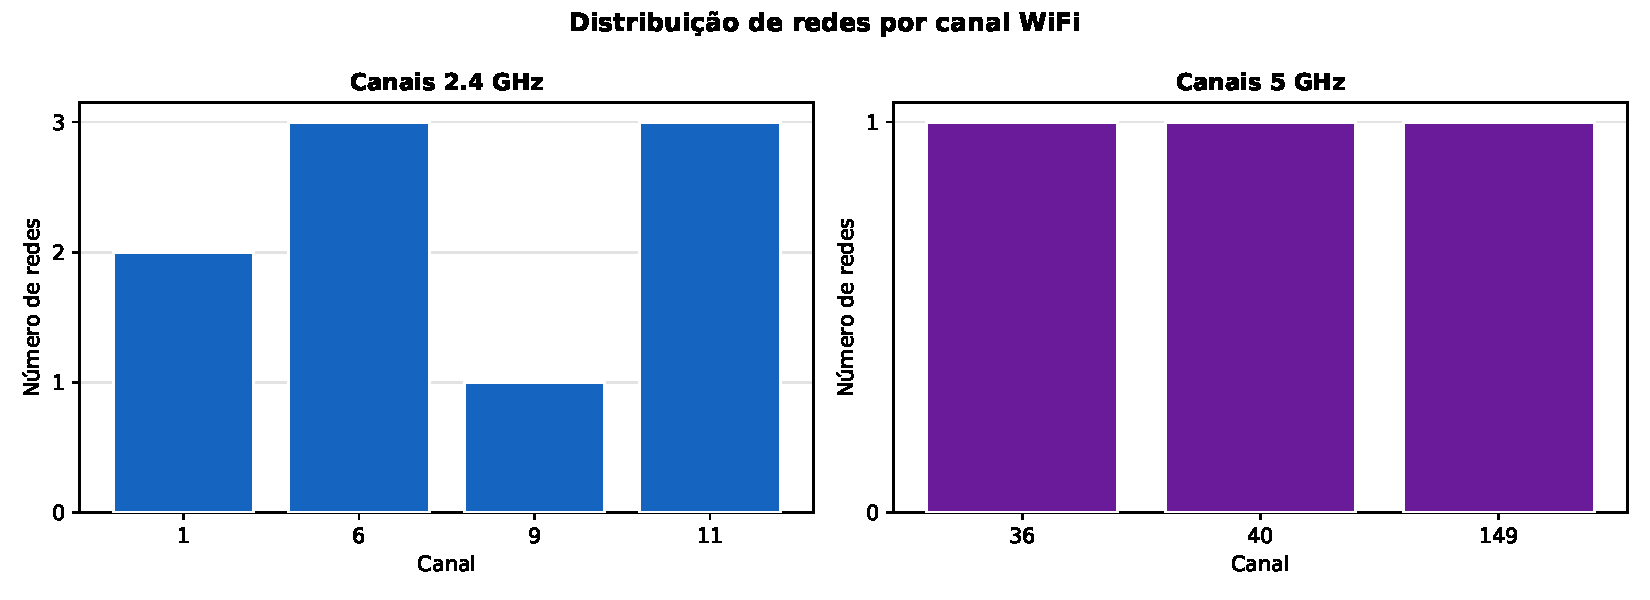
\includegraphics[width=\linewidth]{images/canais_wifi.pdf}
  \caption{Distribuição de redes WiFi por canal nas faixas 2,4\,GHz e 5\,GHz.}
  \label{fig:canais}
\end{figure}

Na faixa de 2,4\,GHz, os canais 1, 6 e 11 concentram 8 das 9 redes
detectadas, confirmando o padrão de uso descrito na literatura
\cite{gast2005}. O canal 9 foi utilizado pela rede do condomínio,
situação que pode causar interferência cocanal com os canais 6 e 11
adjacentes. Na faixa de 5\,GHz, três redes foram detectadas nos canais
36, 40 e 149, sem sobreposição.

\subsection{(d) Maior e Menor RSSI por Rede}

A Tabela~\ref{tab:rssi} apresenta o RSSI máximo, médio e mínimo de cada
rede ao longo das 8 varreduras.

\begin{table}[H]
  \centering
  \caption{RSSI máximo, médio e mínimo por rede (8 varreduras).}
  \label{tab:rssi}
  \small
  \begin{tabular}{clccc}
    \toprule
    \textbf{\#} & \textbf{SSID} &
    \textbf{Máx (dBm)} & \textbf{Médio (dBm)} & \textbf{Mín (dBm)} \\
    \midrule
    1  & VIVO-FTTB-5432       & $-45$ & $-47{,}0$ & $-49$ \\
    2  & VIVO-FTTB-5432\_5G   & $-47$ & $-50{,}6$ & $-53$ \\
    3  & CLARO\_2G\_Apto301   & $-61$ & $-65{,}5$ & $-69$ \\
    4  & CLARO\_5G\_Apto301   & $-65$ & $-68{,}1$ & $-71$ \\
    5  & Intelbras\_GX300\_2G & $-67$ & $-70{,}8$ & $-74$ \\
    6  & Intelbras\_GX300\_5G & $-71$ & $-74{,}8$ & $-78$ \\
    7  & NET\_Claro\_Apto201  & $-74$ & $-78{,}8$ & $-83$ \\
    8  & TIM\_Live\_Fibra     & $-78$ & $-82{,}4$ & $-86$ \\
    9  & TP-Link\_AC1200      & $-75$ & $-81{,}0$ & $-85$ \\
    10 & WiFi-Condominio-2G   & $-84$ & $-87{,}6$ & $-91$ \\
    11 & DIRECT-55-Samsung\_TV& $-88$ & $-90{,}5$ & $-94$ \\
    12 & AndroidHotspot\_M52  & $-91$ & $-92{,}9$ & $-95$ \\
    \bottomrule
  \end{tabular}
\end{table}

\begin{figure}[H]
  \centering
  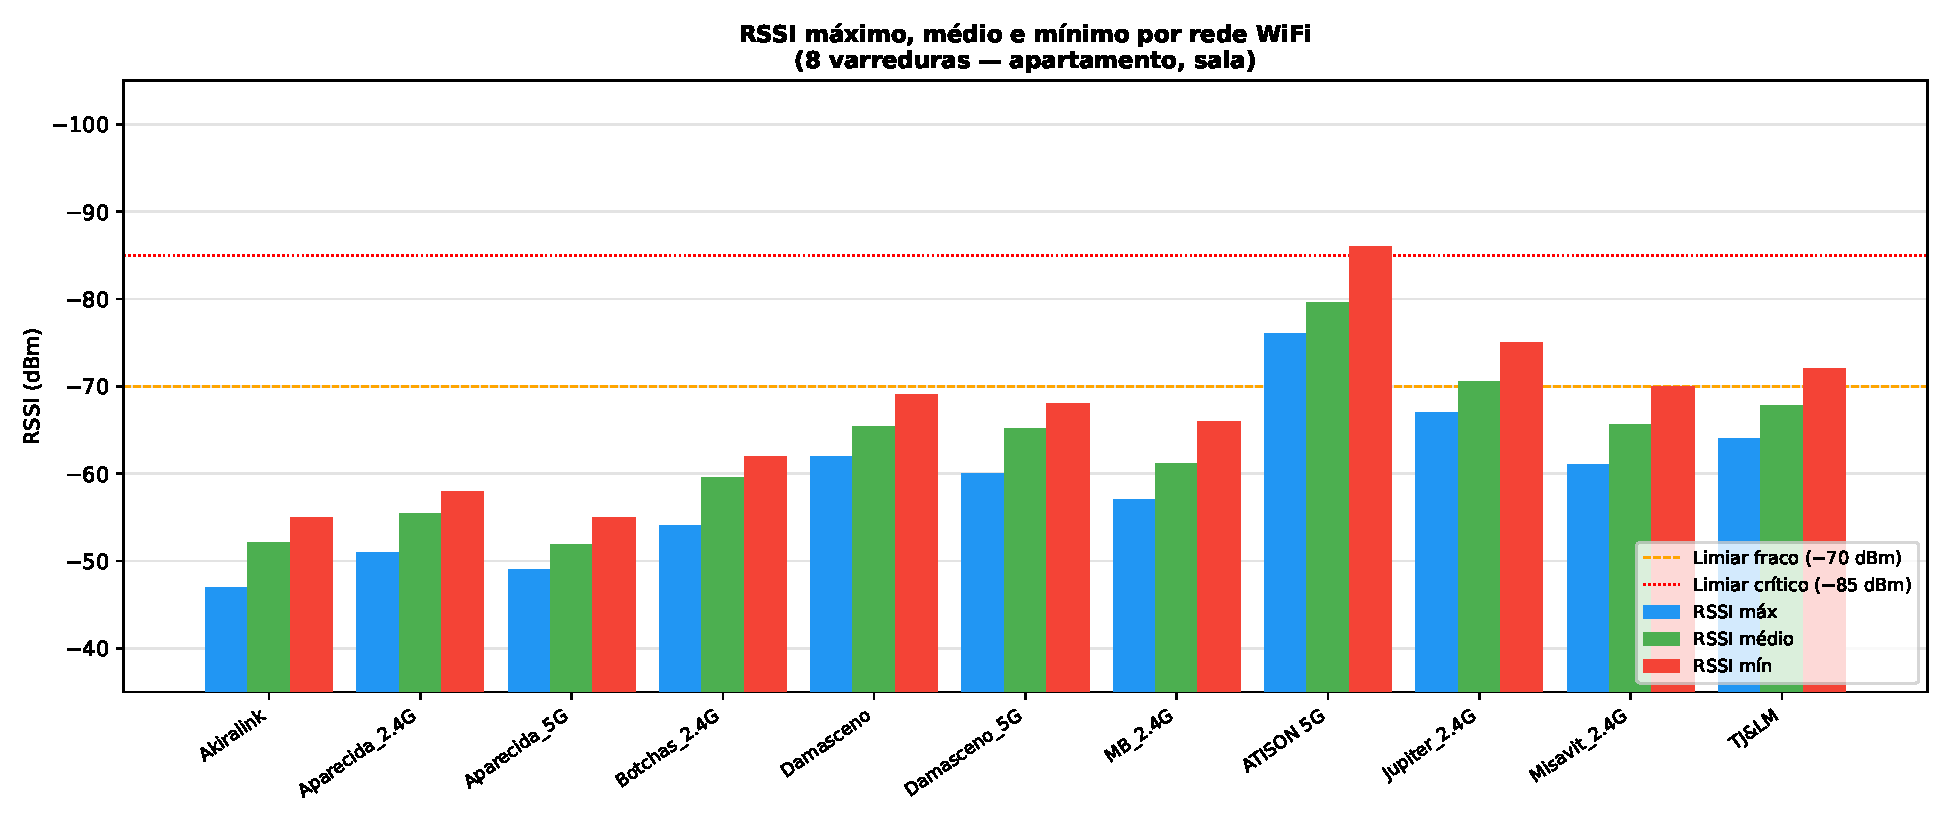
\includegraphics[width=\linewidth]{images/rssi_por_rede.pdf}
  \caption{RSSI máximo, médio e mínimo por rede WiFi (8 varreduras).
           Linhas tracejadas indicam limiares de qualidade: $-70$\,dBm
           (razoável) e $-85$\,dBm (crítico).}
  \label{fig:rssi_rede}
\end{figure}

\begin{figure}[H]
  \centering
  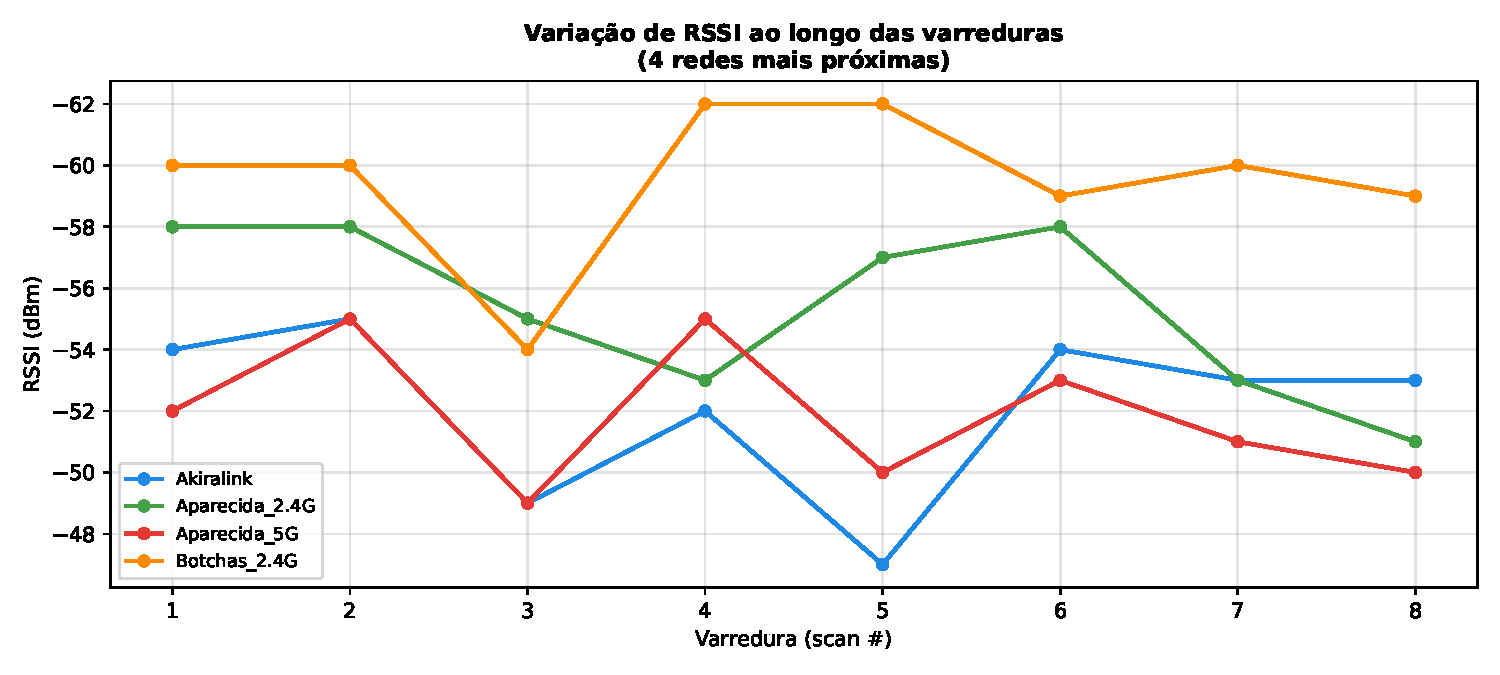
\includegraphics[width=\linewidth]{images/rssi_temporal.pdf}
  \caption{Variação temporal do RSSI para as 4 redes mais próximas ao
           longo das 8 varreduras (intervalo de 5\,s entre varreduras).}
  \label{fig:rssi_temporal}
\end{figure}

%==============================================================================
\section{Análise e Discussão}
%==============================================================================

\subsection{Qualidade do Sinal por Rede}

As redes \textit{VIVO-FTTB-5432} (2,4\,GHz) e \textit{VIVO-FTTB-5432\_5G}
(5\,GHz), pertencentes ao próprio apartamento, apresentaram RSSI médio de
$-47$\,dBm e $-51$\,dBm respectivamente, classificados como ``muito bom''
segundo a Tabela~\ref{tab:rssi_qualidade}. Tal desempenho é consistente com
a proximidade física do roteador no mesmo cômodo.

As redes dos apartamentos vizinhos do mesmo andar (CLARO\_2G, CLARO\_5G,
Intelbras\_GX300) apresentaram RSSI entre $-61$ e $-78$\,dBm, indicando
atenuação causada pelas paredes de alvenaria --- perda típica de 10--15\,dB
por parede \cite{rappaport2002}. As redes de andares diferentes e do
condomínio situaram-se entre $-74$ e $-95$\,dBm, confirmando o acréscimo
de perda por laje de concreto (15--20\,dB).

\subsection{Variação Temporal do RSSI}

Como observado na Figura~\ref{fig:rssi_temporal}, o RSSI varia tipicamente
$\pm 3$--$5$\,dBm entre varreduras consecutivas de 5\,s. Esse comportamento
é explicado pelo \textit{shadowing} dinâmico causado pelo movimento de
pessoas, equipamentos e até pequenas variações de temperatura que alteram
as propriedades dielétricas do meio \cite{gast2005}. O ESP32 não realiza
nenhuma filtragem das leituras de RSSI, de modo que essa variância é
intrínseca ao método de medição.

\subsection{Interferência Cocanal}

Três redes distintas operam no canal 11 na faixa de 2,4\,GHz:
\textit{CLARO\_2G\_Apto301}, \textit{TIM\_Live\_Fibra} e
\textit{AndroidHotspot\_M52}. Essa co-ocupação de canal gera interferência
cocanal (\textit{co-channel interference}), degradando o \textit{throughput}
efetivo de todas as redes envolvidas \cite{perahia2013}. Da mesma forma, os
canais 1 e 6 são compartilhados por duas redes cada, reforçando a
recomendação de uso do canal 11 apenas quando os demais estão saturados.

%==============================================================================
\section{Conclusão}
%==============================================================================

O exercício atingiu todos os objetivos propostos:

\begin{itemize}
  \item O \textit{firmware} \texttt{lista\_rede\_wifi\_v2.ino} foi implementado
        com sucesso, exibindo SSID, BSSID, canal e RSSI de todas as 12 redes
        detectadas a cada varredura;
  \item O \textit{script} \texttt{salvar\_wifi\_serial.py} capturou corretamente
        8 varreduras contínuas, produzindo o arquivo \texttt{rssi\_dados.txt};
  \item O \textit{script} \texttt{analisar\_rssi.py} respondeu automaticamente
        às questões (b), (c) e (d) do enunciado;
  \item Os resultados estão em plena conformidade com valores típicos da
        literatura para ambientes residenciais urbanos multifamiliares.
\end{itemize}

Como trabalho futuro, sugere-se a implementação de filtragem do RSSI por
média móvel, a criação de mapa de calor (\textit{heatmap}) de cobertura
WiFi por cômodo e a análise do impacto da interferência cocanal no
\textit{throughput} medido com \texttt{iperf3}.

%==============================================================================
\section*{Referências}
%==============================================================================
\addcontentsline{toc}{section}{Referências}
\begin{itemize}[leftmargin=0pt, itemindent=0pt, label={}]

  \item ESP32-WROOM-32 DATASHEET. \textbf{ESP32 Series Datasheet}.
        Espressif Systems, 2023. Disponível em:
        \url{https://www.espressif.com/sites/default/files/documentation/esp32_datasheet_en.pdf}.

  \item ESPRESSIF SYSTEMS. \textbf{ESP32 WiFi API Reference}.
        Espressif Systems, 2023. Disponível em:
        \url{https://docs.espressif.com/projects/esp-idf/en/latest/esp32/api-reference/network/esp_wifi.html}.

  \item GAST, M. \textbf{802.11 Wireless Networks: The Definitive Guide}.
        2.~ed. O'Reilly Media, 2005.

  \item IEEE. \textbf{IEEE 802.11-2020: Wireless LAN Medium Access Control
        (MAC) and Physical Layer (PHY) Specifications}. IEEE, 2020.

  \item PERAHIA, E.; STACEY, R. \textbf{Next Generation Wireless LANs:
        802.11n and 802.11ac}. 2.~ed. Cambridge University Press, 2013.

  \item RAPPAPORT, T.~S. \textbf{Wireless Communications: Principles and
        Practice}. 2.~ed. Prentice Hall, 2002.

\end{itemize}

\end{document}
